\begin{savequote}[8cm]
Far out in the uncharted backwaters of the unfashionable end of the western spiral arm of the Galaxy lies a small unregarded yellow sun. Orbiting this at a distance of roughly ninety-two million miles is an utterly insignificant little blue green planet whose ape-descended life forms are so amazingly primitive that they still think digital watches are a pretty neat idea.
  \qauthor{--- D. Adams, The Hitchhiker's Guide to the Galaxy}
\end{savequote}

\chapter{\label{ch:1-intro}Introduction} 
This chapter explains the background and motivation for my project and introduces the two sub-projects I have been working on for the last year.
\minitoc

\section{Scope of the thesis}

\section{Background}
I am pursuing my graduate studies in Condensed Matter Physics as an Early-Stage Researcher, part of a Marie Skłodowska-Curie Innovative Training Network called \emph{DNA-Robotics}\footnote{\url{https://dna-robotics.eu/}, grant agreement number 765703}. The network consists of the leading European DNA nanotechnology research groups and was formed with the goal of creating a unified framework for integrated biomolecular robotics\cite{dnaroboticsResearch}.

My position, in particular, is assigned to develop standardised techniques for the design and self-assembly of the nanorobotic modules\cite{dnaroboticsESR12}. The original design proposed for the robotic modules was to use cubic DNA origami modules, as shown in Figure \ref{fig:dnaRoboticsHeader}, but the the goals have since broadened to include additional module types. Other Early-Stage Researchers within the network are tasked with developing such modules with either sensoring, actuating or signal processing capabilities. The motivation for developing standardised modules is that they, when proven to work, can be reused in new designs, saving development time and resources.

\begin{figure}
    \centering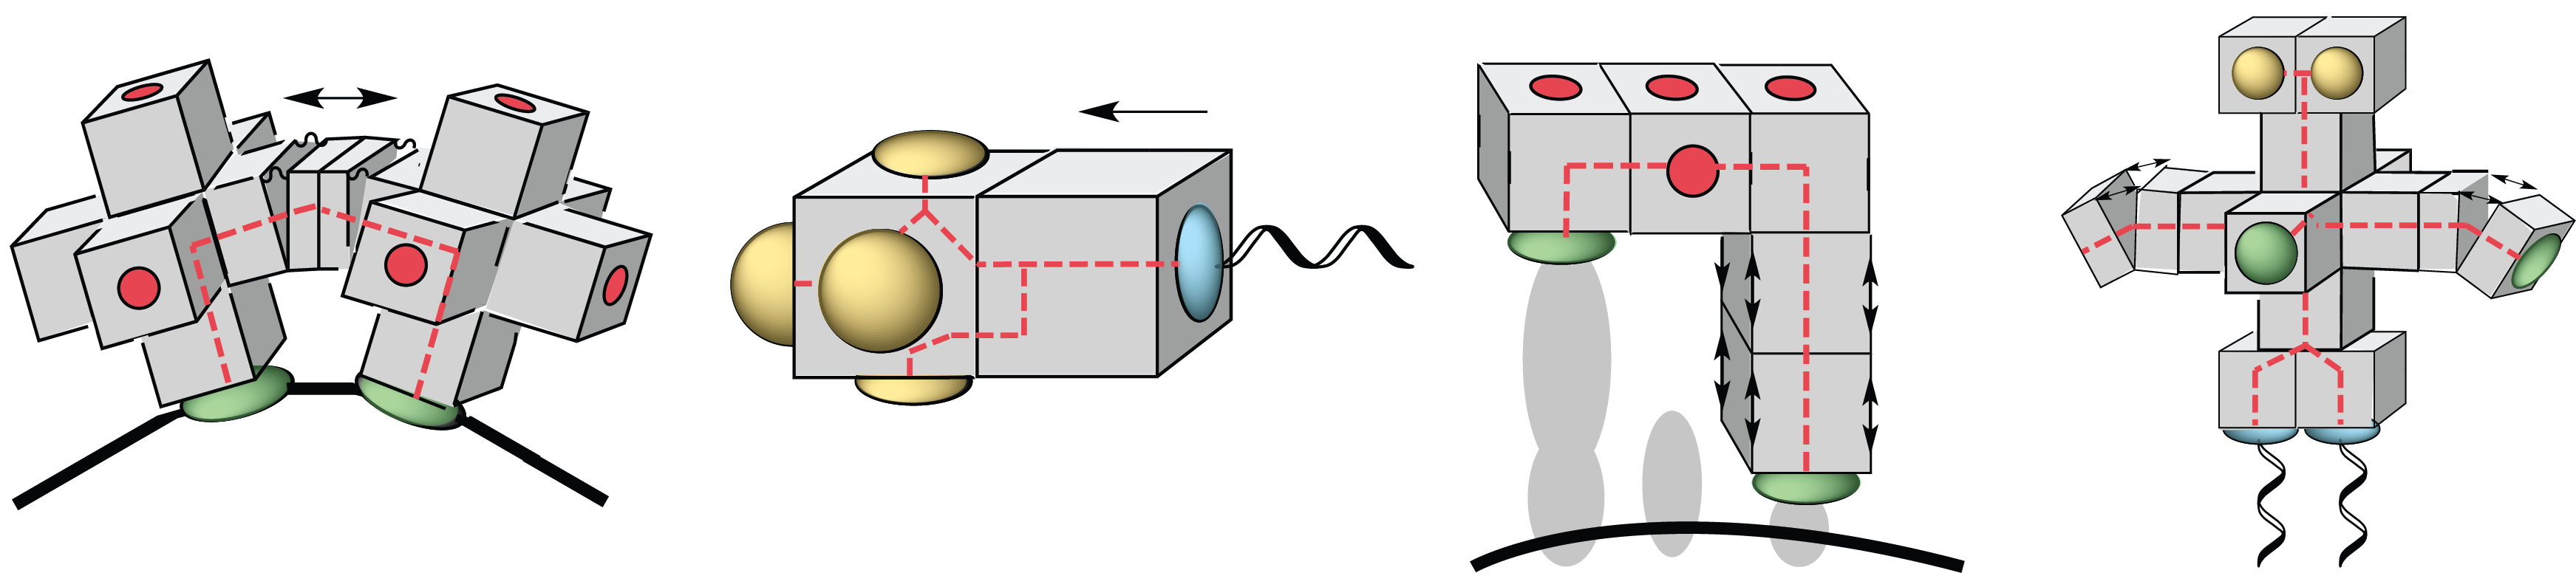
\includegraphics[width=\textwidth]{figures/dnaRoboticsHeader.png} 
    \caption{Conceptual DNA Robotics design. The nanorobots are assembled from standardised cubic modules that functions as sensor, actuators, processors, or structural components. Image adapted from \url{https://dna-robotics.eu/about/}}
    \label{fig:dnaRoboticsHeader}
\end{figure}

As such, my contribution to the network and the field will be a step further in the ongoing effort to find methods for organising matter on the nanoscale.

\subsection{Deoxyribonucleic acid (DNA)}
Deoxyribonucleic acid (DNA)

\subsection{Ribonucleic acid (RNA)}
Ribonucleic acid (RNA) is a molecule

\subsection{DNA origami}

DNA origami\cite{rothemund2006folding} is a popular and proven method for creating larger irregular structures using DNA. The principle behind it, as illustrated in Figure \ref{fig:dnaOrigami}, is to use short staple strands to fold one long viral scaffold strand into the desired structure.

\begin{figure}
    \centering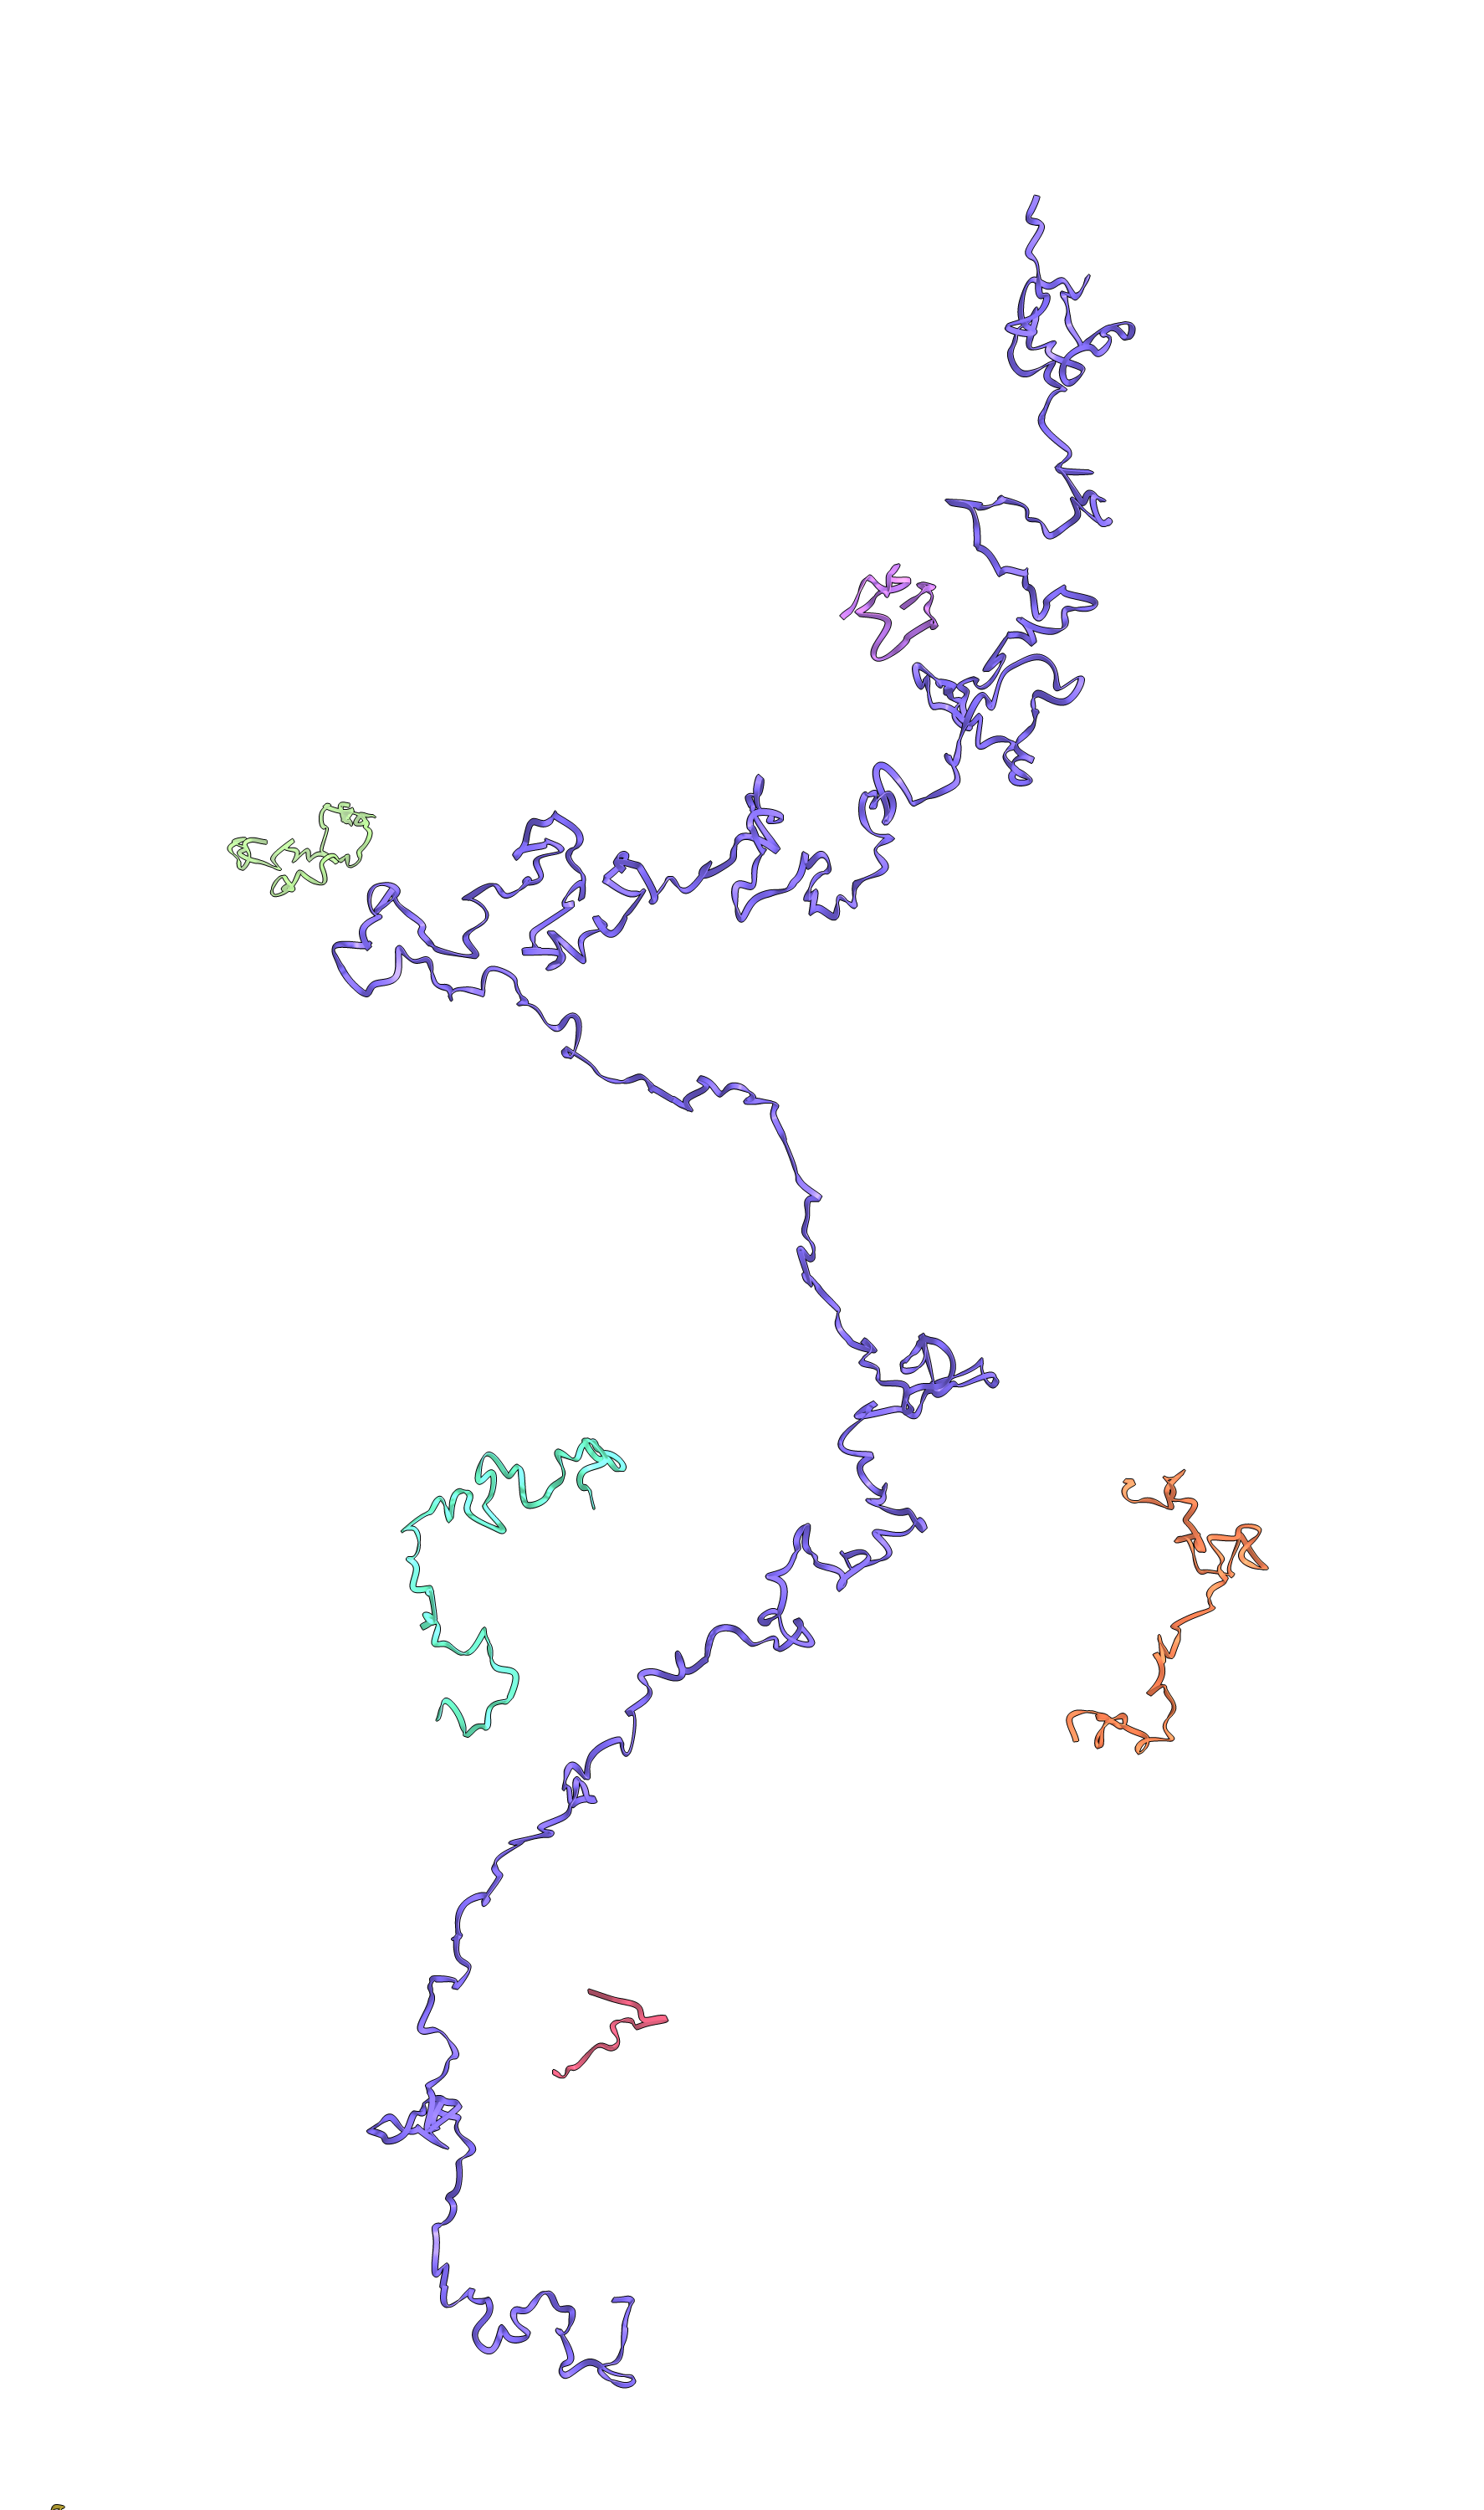
\includegraphics[width=\textwidth/5]{figures/melt/melted.png}\hfill
%    \centering\includegraphics[width=\textwidth/5]{figures/melt/intermediate2.png}\hfill
    \centering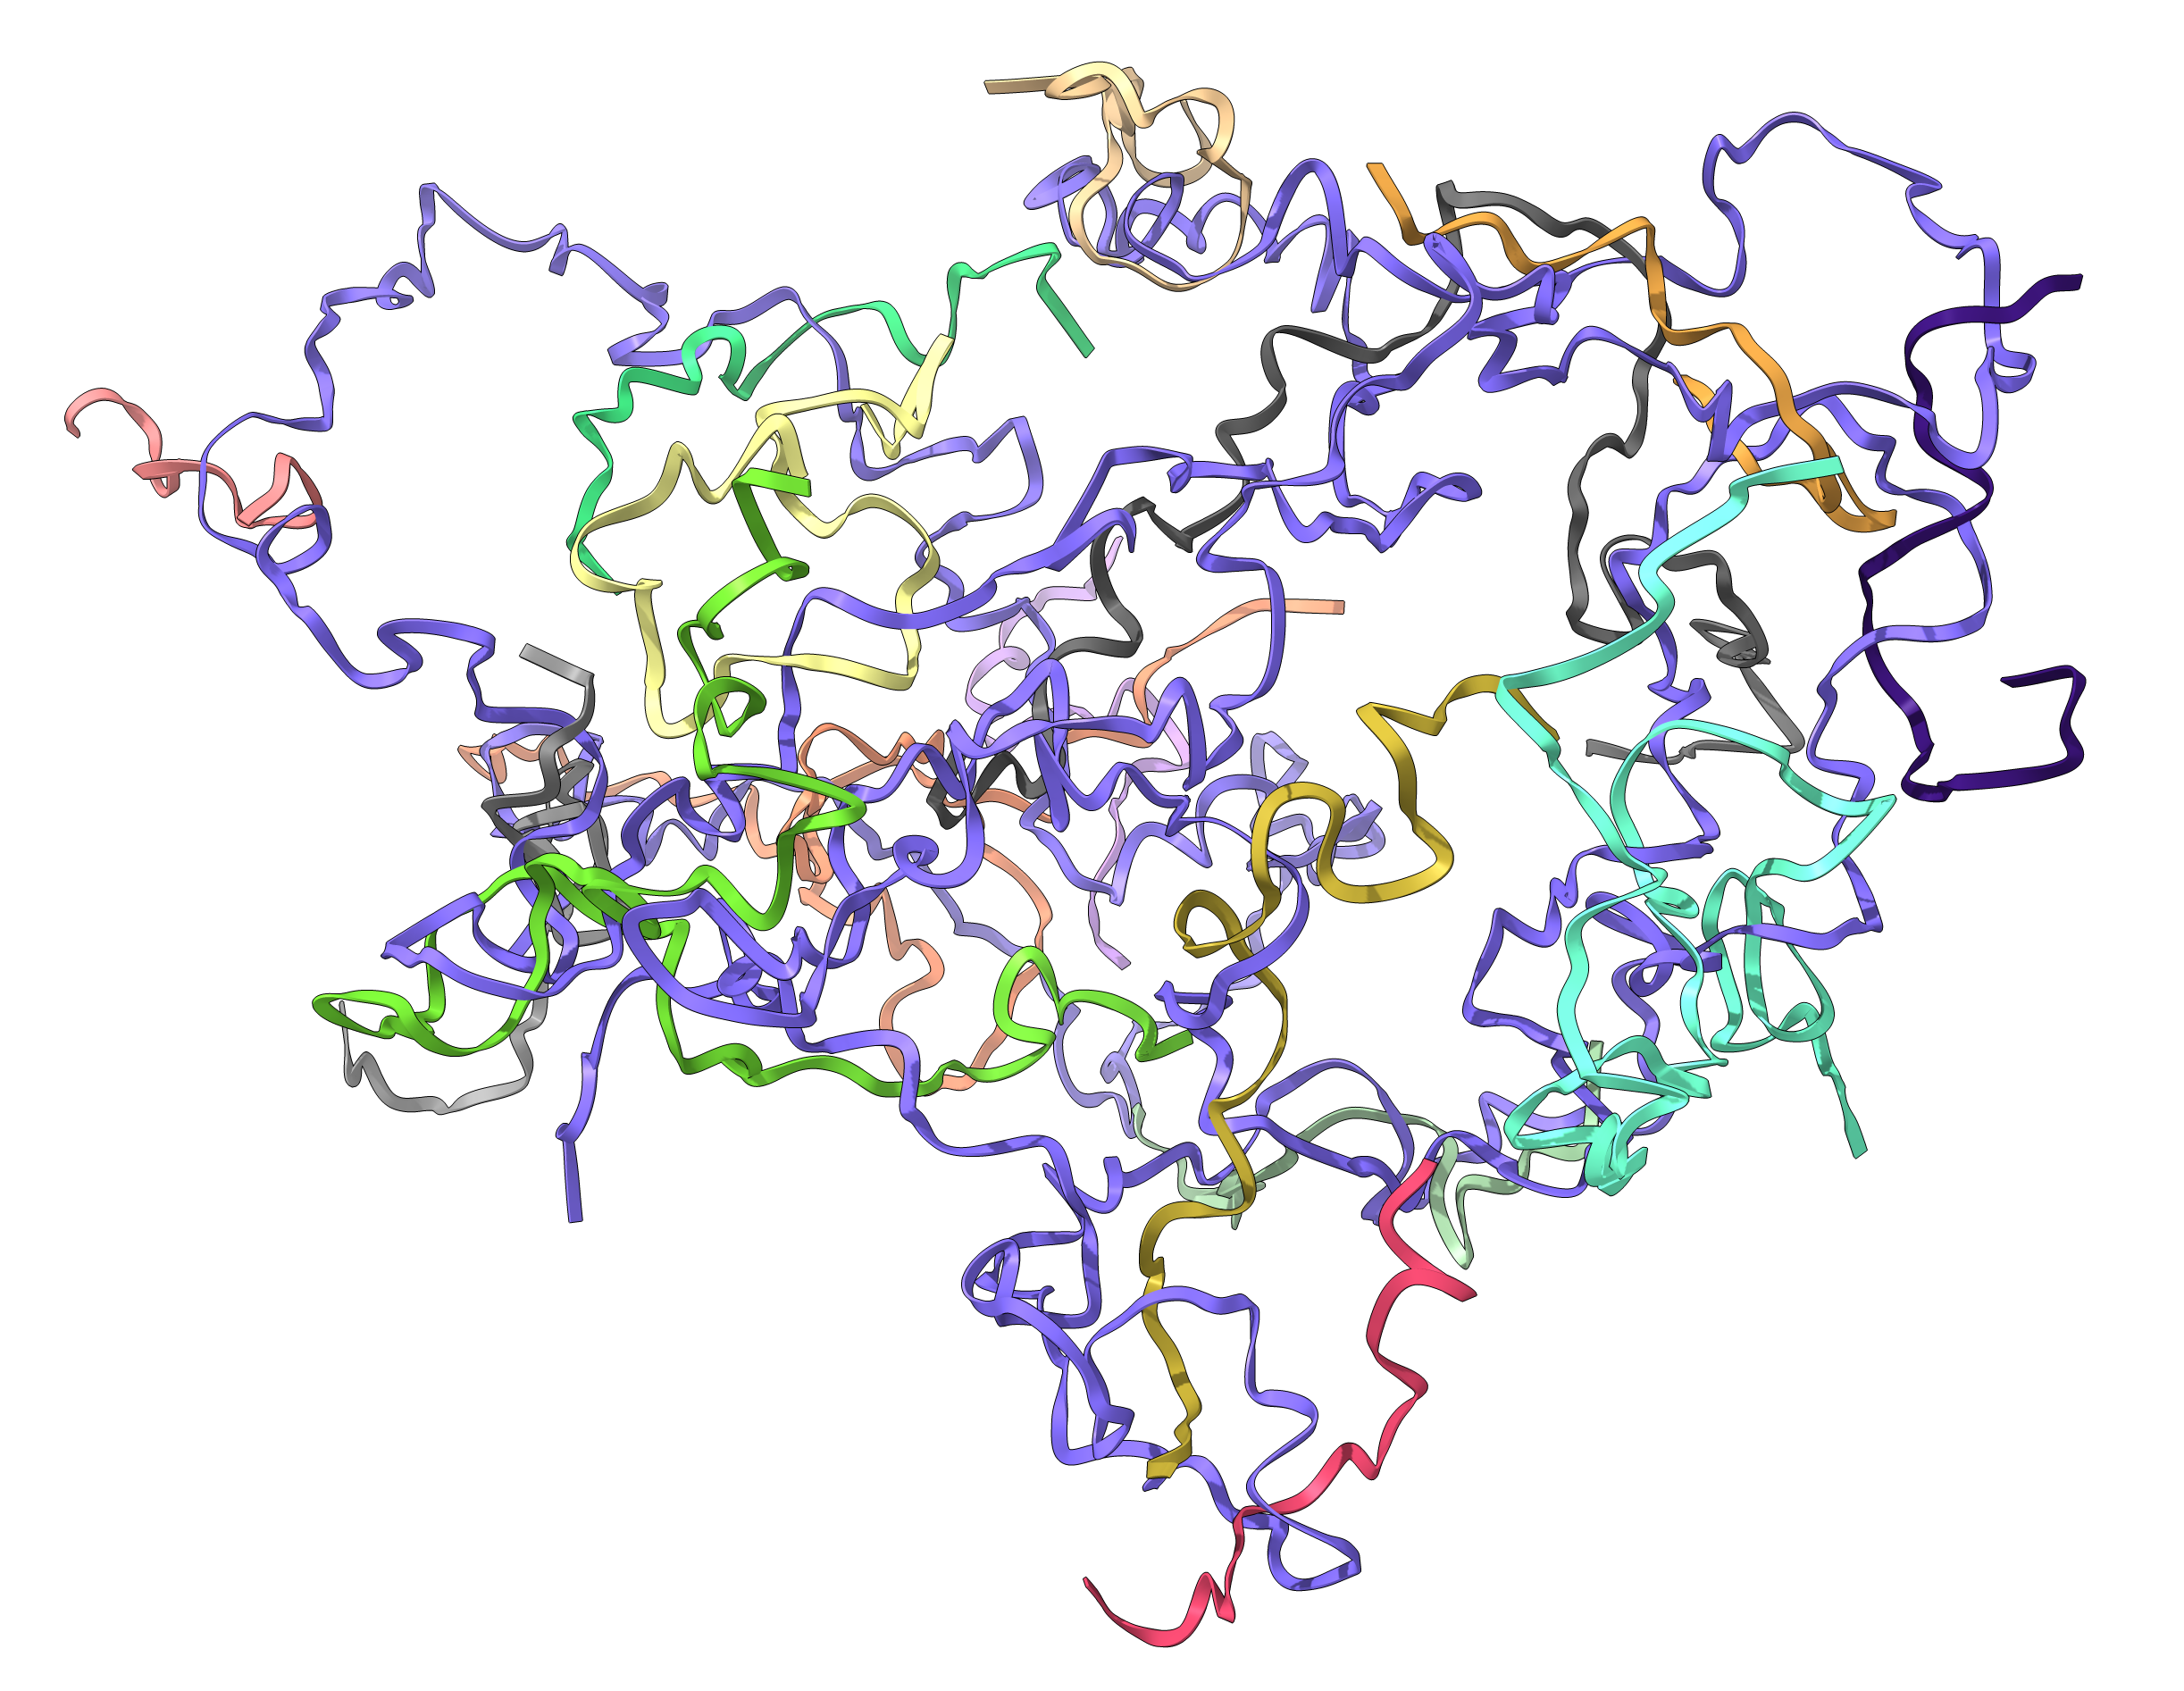
\includegraphics[width=\textwidth/3]{figures/melt/intermediate1.png}\hfill
    \centering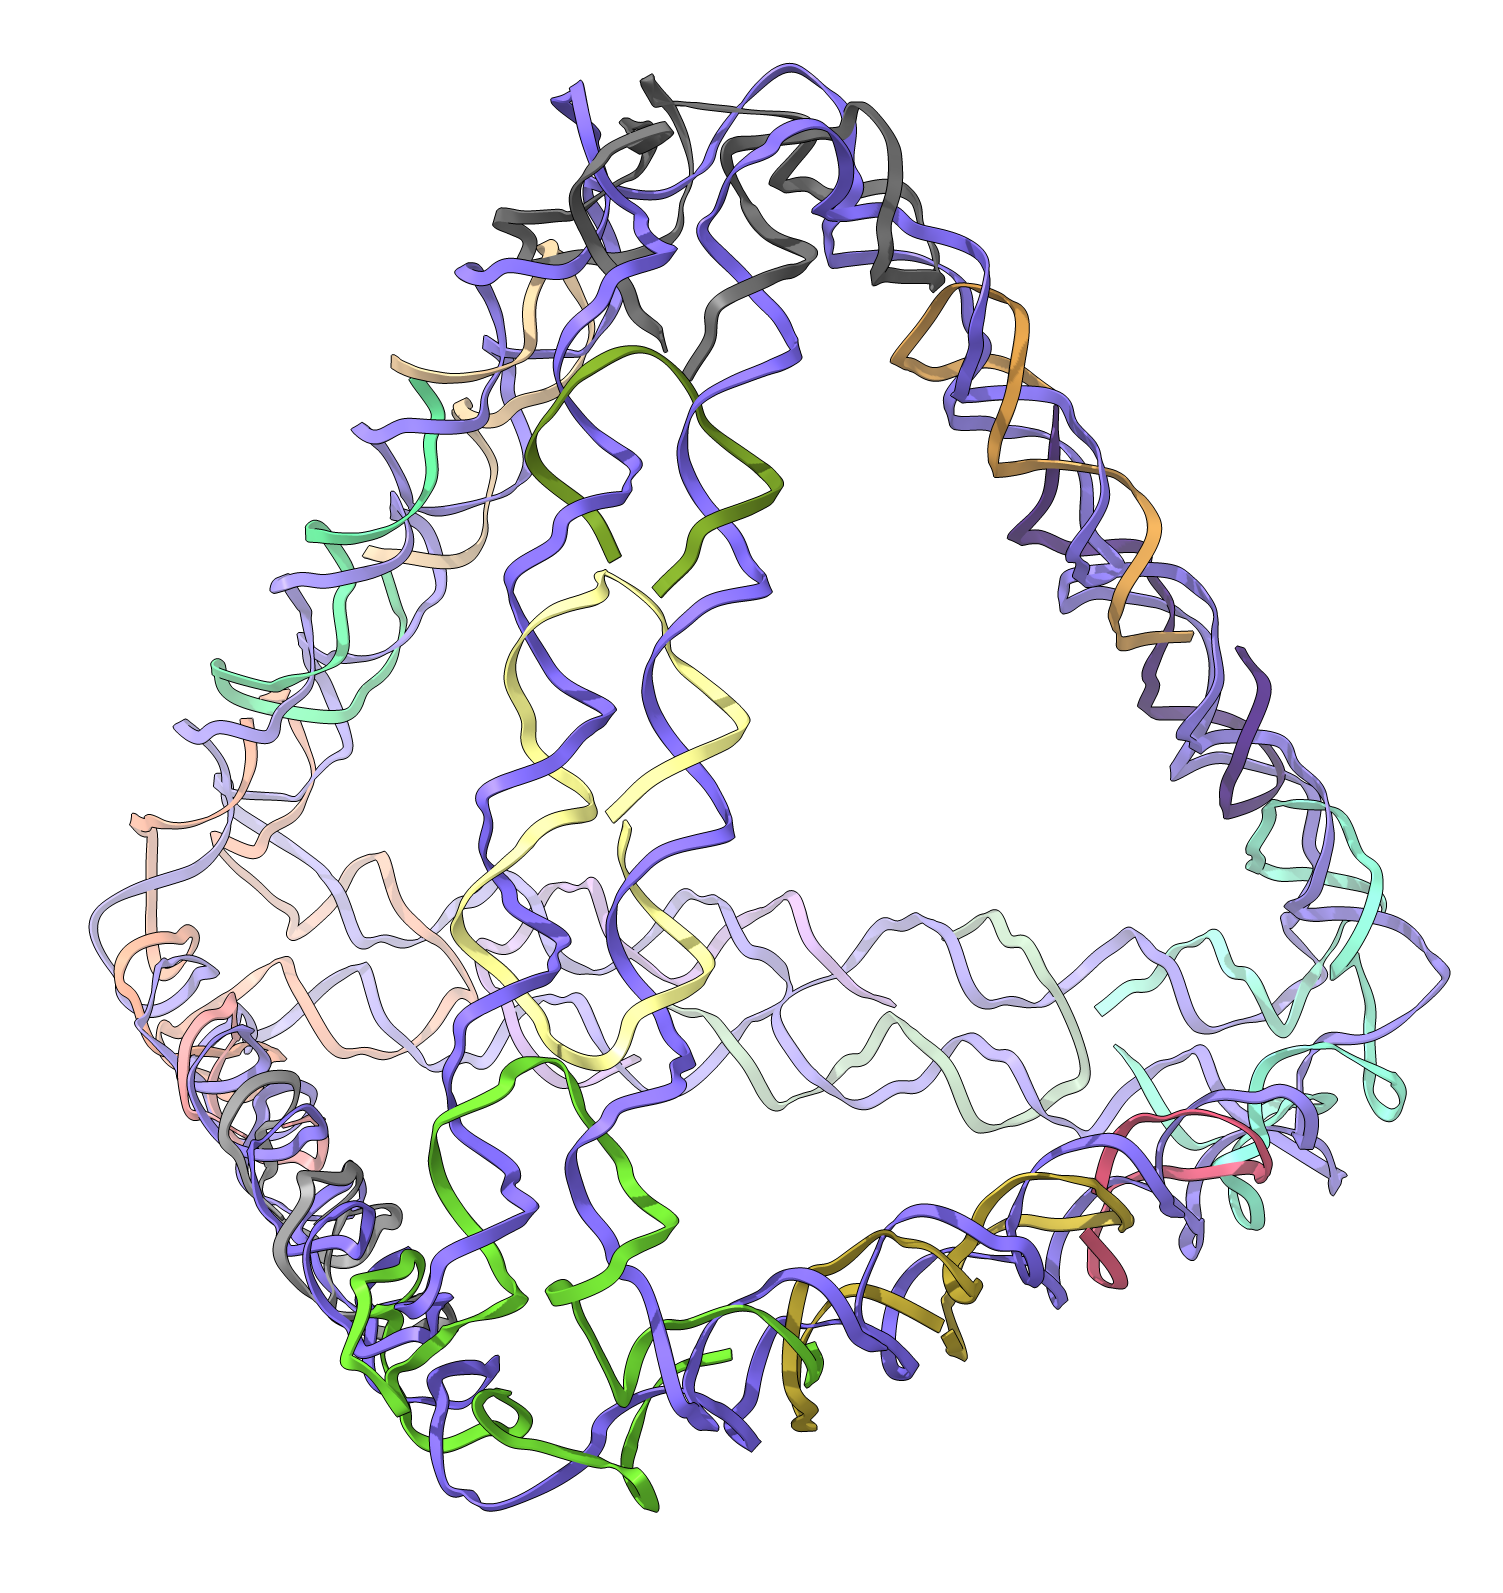
\includegraphics[width=\textwidth/3]{figures/melt/assembled.png}
    \caption{Illustration of DNA origami self-assembly of a tetrahedron. A long scaffold strand (purple), obtained from a virus, is folded into the desired shape by multiple short staple strands binding to complementary domains of the scaffold. Tetrahedron design obtained from \url{https://cando-dna-origami.org/examples/} and melted using oxDNA simulation \cite{ouldridge2010dna}.
    }
    \label{fig:dnaOrigami}
\end{figure}

Using design tools such as caDNAno\cite{douglas2009rapid}, it has become relatively easy to design structures of any given form. However, the size of the origami is limited by the length of the scaffold, which one of the motivations for researchers to investigate modular approaches, as described in Section \ref{sec:experimental_appl}.

\subsection{RNA origami}

Another possible building material investigated by the DNA robotics network is RNA. While DNA folding is easier to predict, the fact that RNA is more reactive also offers the possibility of a more useful structure; for example by incorporating aptamers, enzymes and other such functionalities\cite{guo2010emerging}.
Geary, et al., from the Andersen lab in Aarhus, demonstrated a method\cite{geary2014single, sparvath2017computer} for co-transcriptionally folded RNA origami in 2014, which also enables folding \emph{in vivo}. Using RNA origami, they were able to develop RNA tile modules, connecting through kissing-loop interactions. The Andersen lab is one of the network partners and I have spent a two-months secondment there working with their RNA origami method.

% "The emerging field of RNA nanotechnology121 might seem more promising in this regard because RNA is readily transcribed into a single strand in cells, which can be directly folded into a programmed nanostructure"
% https://www.nature.com/articles/nnano.2011.187

In order achieve my goal of improving the design of modular robotic structures, simulation tools are needed to analyse the assembly of both the complete structures and of each module. During the past year, I have been working with two related sub-projects to solve both those needs, each described in the following two sections.

